\subsection{Why performance collapses over time (E7)}
\label{sec:drift}

\begin{figure}[t]
  \centering
  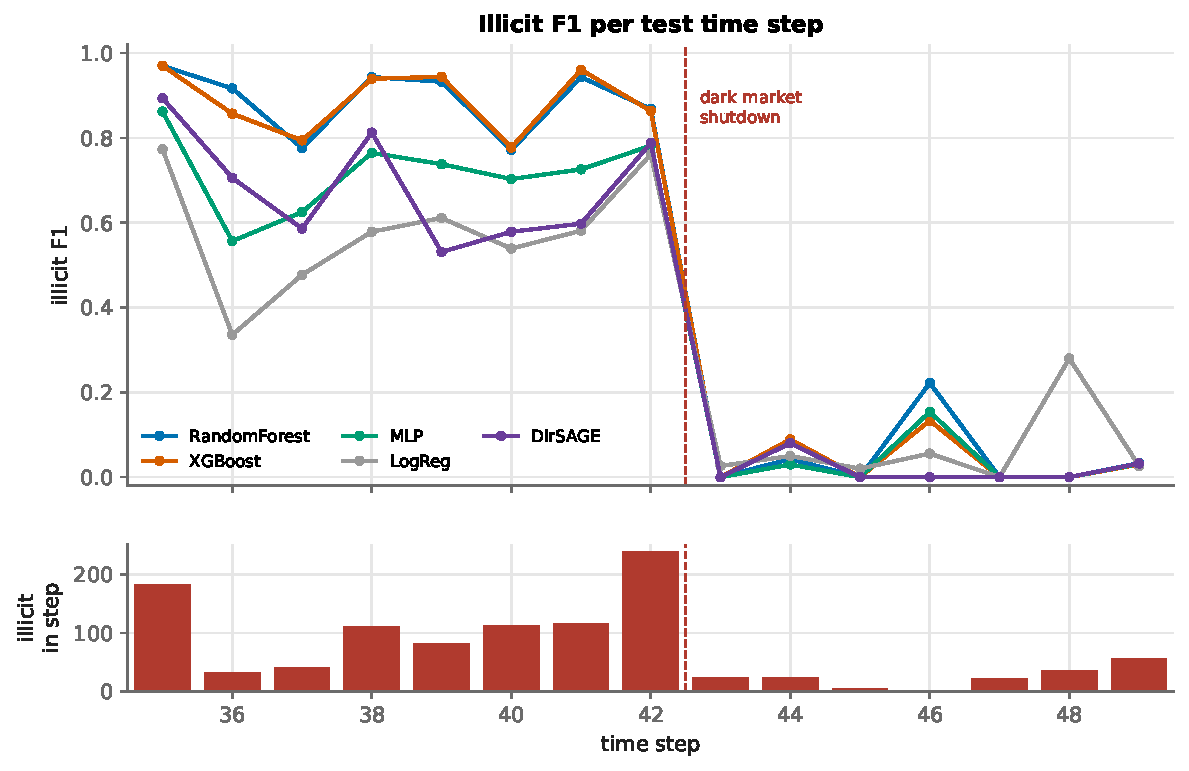
\includegraphics[width=\columnwidth]{../reports/figures/e07_f1_per_step.pdf}
  \caption{Illicit F1 per test step (top) and number of illicit transactions per
  step (bottom). Every model collapses at the dark market shutdown.}
  \label{fig:perstep}
\end{figure}

Fig.~\ref{fig:perstep} is the most important figure of this study. Before the
dark market shutdown, the tree models reach a mean per-step F1 of
\DriftRFPre{} (Random Forest) and \DriftXGBPre{} (XGBoost); from step 43 on they
reach \DriftRFPost{} and \DriftXGBPost{}. No model, linear, tree, neural or
graph, survives the event. The pooled test F1 of about 0.8 is therefore an
average of two regimes: near-perfect detection of a known kind of crime, and
almost no detection of the kind that replaced it.

\textbf{A hidden clock.} Before asking what changed, we had to remove something
that changes for everyone. \ClockCount{} of the aggregated features
(\ClockList{}) rise almost monotonically with time ($|\rho|\geq\ClockMinRho{}$
with the time step on the training steps). They work like the time-step column we
removed: any two periods can be told apart through them. Removing them from the
models changes nothing (F1 difference \ClockAblRFFoneDiff{}, $p\ClockAblRFFoneP{}$
for Random Forest), so the trees do not exploit them, but they must be removed
before any drift analysis.

\textbf{The illicit population changed; the licit one barely did.} Without the
clock features, we compare each feature's distribution before and after step 43
with a Kolmogorov--Smirnov test, separately for each class. For illicit
transactions, \AdvIllicitKSShare{} of the features shift strongly (KS
statistic $>0.3$); for licit transactions, only \AdvLicitKSShare{}. A classifier
can still separate the two periods within either class (AUC
\AdvIllicitAUC{} and \AdvLicitAUC{}), because a few slowly drifting features
remain. So the per-feature view is the informative one: almost every illicit
feature moved, while the licit population stayed largely the same.

\textbf{The new illicit transactions look licit.} For each illicit test
transaction we compare the distance to its nearest illicit training transaction
with the distance to its nearest licit one (Fig.~\ref{fig:novelty}). Before the
shutdown, \NovelPre{} are closer to licit traffic; after it, \NovelPost{}. A
model that learned what illicit activity \emph{used to} look like has nothing to
recognise.

\begin{figure}[t]
  \centering
  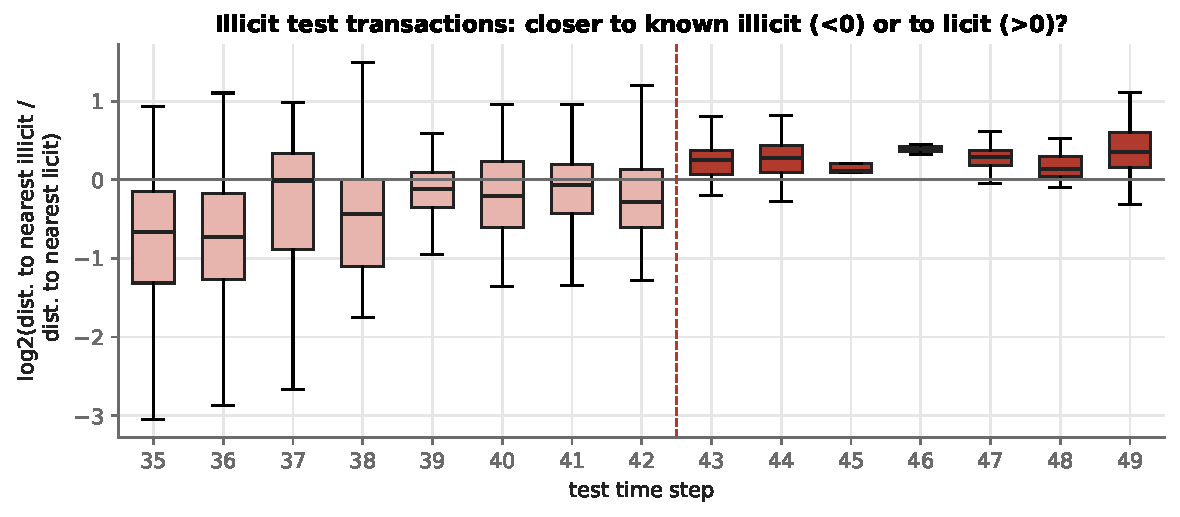
\includegraphics[width=\columnwidth]{../reports/figures/e07_novelty.pdf}
  \caption{Relative distance of illicit test transactions to the nearest
  illicit vs.\ nearest licit training transaction (log scale; above 0 means closer
  to licit). Clock features removed.}
  \label{fig:novelty}
\end{figure}

\textbf{Retraining helps only a little.} If the model is retrained on every
labelled step before scoring the next one (Fig.~\ref{fig:walk}), F1 after the
shutdown rises from \WFStaticPost{} to \WFExpandingPost{} (expanding window) or
\WFSlidingPost{} (last 10 steps), recovering mostly in the last step, once
enough new illicit examples have been labelled. Before the shutdown, retraining
changes little (\WFStaticPre{} vs \WFExpandingPre{}). This confirms and quantifies
the observation of Weber et al.: the bottleneck after a regime change is
labels for the new behaviour, not the model.

\begin{figure}[t]
  \centering
  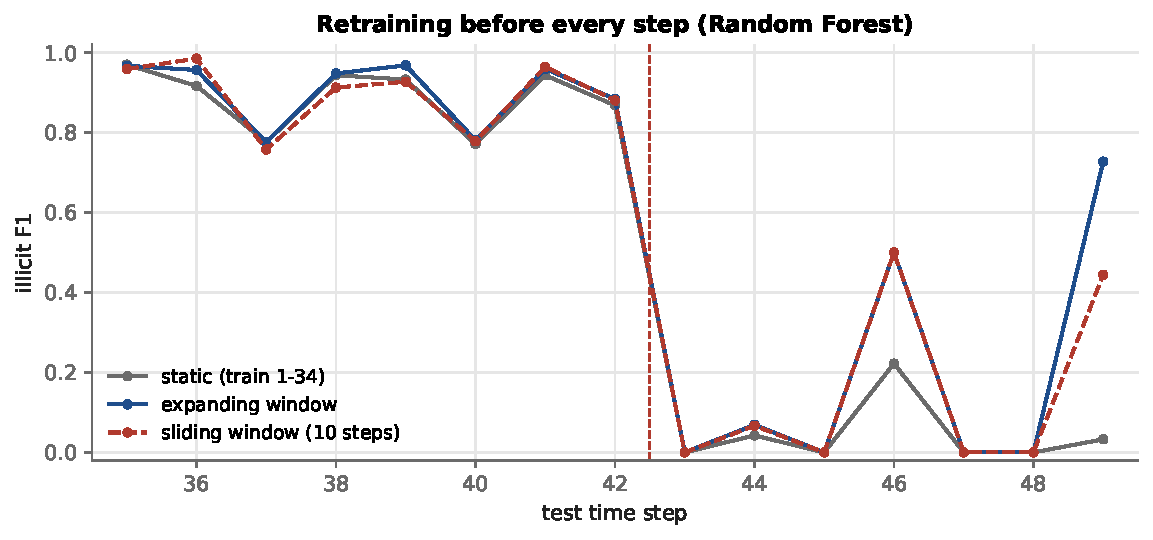
\includegraphics[width=\columnwidth]{../reports/figures/e07_walk_forward.pdf}
  \caption{Random Forest retrained before every test step on all earlier
  labelled steps (expanding) or the last 10 (sliding), vs.\ trained once.}
  \label{fig:walk}
\end{figure}
